\graphicspath{{chapters/05/}}
\chapter{Spatial omics}

\hypertarget{spatial-transcriptomics}{%
\section{Spatial
Transcriptomics}\label{spatial-transcriptomics}}

A range of methods for \textbf{quantifying RNAs} in \textbf{specific
locations} on histological sections \emph{``retaining information on
spatial context''.} Important criteria:

\begin{itemize}
\tightlist
\item
  \emph{How many RNAs?} → throughput
\item
  \emph{At which resolution?} → the resolution is the unit of space that
  can be discriminated in the image. We cannot have a grid perfectly
  adapting to single cells, so we will observe pieces of different cells
  rather than single cells.
\end{itemize}

If we look at the evolution of main ST platforms, we observe a
correspondence with single cell techniques with a 4-5 years gap.

The main ST approaches can be divided into:
\begin{enumerate}
\def\labelenumi{\arabic{enumi}.}
\tightlist
\item
  \emph{imaging based methods}: read out by microscopy e.g.~multiplexed
  FISH

  \begin{itemize}
  \tightlist
  \item
    Pros: high resolution, depending on the microscope
  \item
    Cons: low coverage or low number of RNAs, need to design target
    probes (not possible to have more than 10 fluorophores)
  \end{itemize}
\item
  \emph{sequencing based methods}: spatial barcoding, read out by
  sequencing - more similar to single cell approaches. The cells are
  placed on a plate covered with adapters (UMI + polyA sequence
  capturing mRNAs different according to the location).

  \begin{itemize}
  \tightlist
  \item
    Pros: high coverage
  \item
    Cons: low resolution
  \end{itemize}
\end{enumerate}

\hypertarget{sequencing-based-methods}{%
\section{Sequencing-based methods}\label{sequencing-based-methods}}

Sequencing based spatial stranscriptomic methods all rely on the idea of 
barcoding the molecules in the original tissue using some in situ technique,
and then to study those molecules using NGS. (The read itself will contain
both the RNA sequence and some barcode sequence that defines the position in
the tissue of origin).

Sequencing-based spatial transcriptomics methods can be broadly divided into 
four main classes, depending on the strategy used to perform the in situ 
barcording. The barcoding strategy also affects the spatial resolution of the 
technique which can range from 55 $\mu m$ spots to 0.5 $\mu m$ spots. 

These techiques, sorted from lowest to highest resolution are:
\begin{itemize}
\tightlist
\item 
  \textbf{10X Visium platform} (2019), which is the optimized version of 
  \textbf{spatial transcriptomics} (2016)
\item
  \textbf{Deterministic barcoding in tissue} (2020)
\item 
  \textbf{Slide-seq} (2019)
\item
  \textbf{Seq-scope} (2021)
\end{itemize}

\textbf{NOTE}: Resolution order and chronological order do NOT match.

These techiniques:
\begin{itemize}
\tightlist
\item
  Allow to analyze thousands of RNAs and allow for unbiased capture. In 
  general though, only poly-A transcripts are analyzed.
\item
  Do not have high-enough resolution to allow for cellular, or subcellular,
  level analysis (unique exception being Scope-seq).
\end{itemize}

\hypertarget{spatial-transcriptomics-2016}{%
\subsection{Spatial transcriptomics
(2016)}\label{spatial-transcriptomics-2016}}

Spatial transcriptomics (ST) is the first sequencing based spatial technique.
Distilling the procedure into its main steps:
\begin{itemize}
\tightlist
\item 
  Create an array on which probes have been printed in about one thousand 
  spots of 100 $\mu m$ diameter, and with center-to-center distance of 200 
  $\mu m$. The probes are composed of cleavage site (to detach the probes 
  from the slide), amplification and sequencing handle, spatial barcode, 
  unique molecule identifier (UMI), mRNA capture region. Notice that \emph{(a)}
  the amplification and sequencing handle is obviously shared by all probes, 
  \emph{(b)} the spatial barcode is shared by all probes in the same spot, 
  \emph{(c)} the UMI is different for all probes in a spot, but probes from
  different spots can have the same UMI (since the combination with the spatial
  barcode still keeps the probes distinct).
\item 
  Place the tissue section on top of the array and perform any required 
  imaging step (H\&E staining, FISH) to acquire an histological image on 
  which to project the spatial data.
\item
  Permeabilize the cells. In the original paper adult mouse olfactory bulb 
  was used since it is a brain region with clear histological landmarks and 
  gene expression reference data.
\item 
  The polyadenilated RNAs hybridize with the probes directly beneath.
\item 
  The hybridized probes can be removed from the array and can be used to 
  construct a standard NGS library. The final reads will still contain the 
  spatial barcode, therefore allowing to map the reads to the original spot on 
  the array.
\end{itemize}

Given the fairly low resolution, multiple cells can be present in the same 
spot; for this reason one cannot be sure that all the transcripts sharing the 
same spatial barcode do indeed belong to the same cell (doublet detection 
and/or deconvolution is needed).

\hypertarget{x-visium-platform-for-spatial-gene-expression-2019}{%
\subsection{10x Visium platform for spatial gene expression
(2019)}\label{x-visium-platform-for-spatial-gene-expression-2019}}

The 10x Visium platform works almost identically to the original spatial 
transcriptomics, it is simply a more optimized and streamlined procedure.

The spot size on the slide is reduced to 55 $\mu m$, the distance between spot 
centers is 100 $\mu m$ and the number of spots is 5000. At this resolution, 1 
to 10 cells could still be in the same spot. Notice that there still is space 
on the array which is not covered by any probe.

This technique works with fresh frozen tissues and, starting from 2022, with 
FFPE (Formalin-Fixed Paraffin-Embedded) tissues (which generally have lower 
quality since the fixation procedure can degrade RNA). 

\begin{figure}
\centering
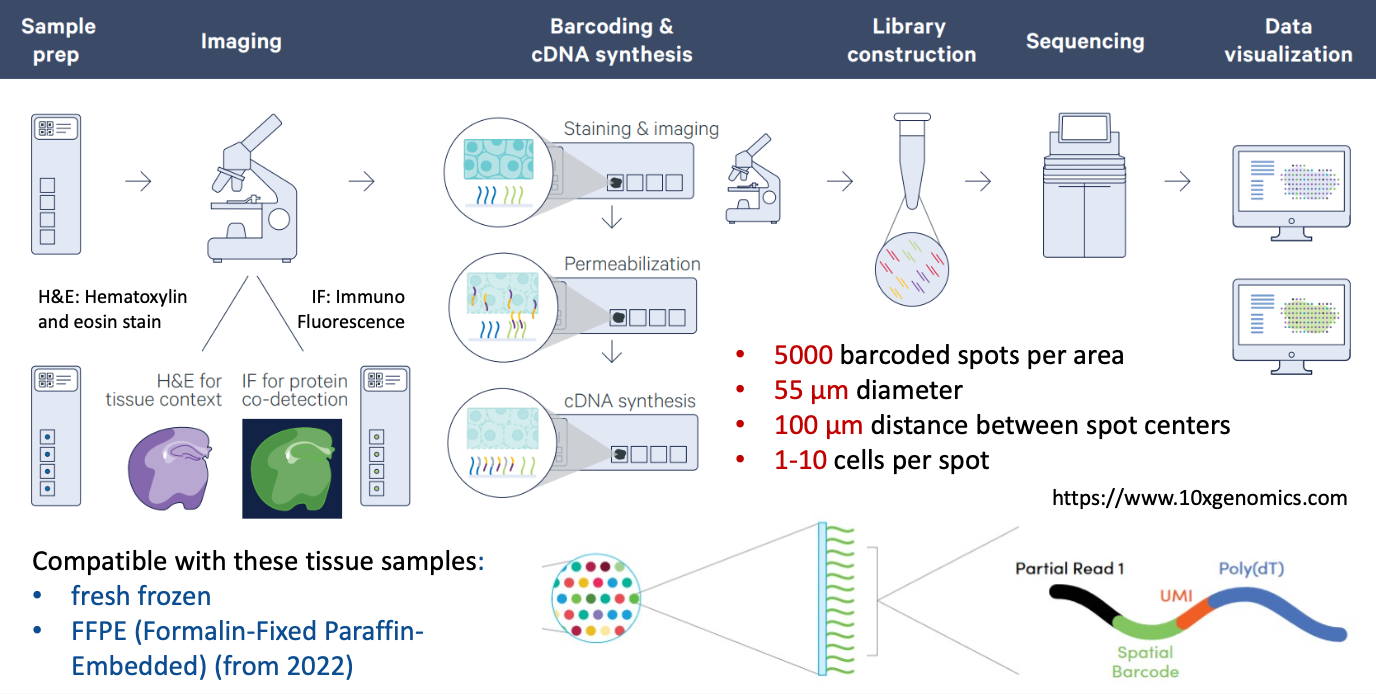
\includegraphics[width=0.5\textwidth]{images/Screenshot.png}
\caption{}
\end{figure}

\hypertarget{sit-2022}{%
\subsection{SiT (2022)}\label{sit-2022}}

Spatial Isoform Transcriptomics (SiT) combines Visium platform with long read
sequencing (Nanopore). The initial steps are the very same ones from the 
Visium platform, but then two different sequencing libraries can be prepared,
a short read 3' library for Illumina sequencing, and a full read length
library for Nanopore sequencing. This allows to analyze spatial distribution
of isoforms (splicing variants).

Given that the first steps are identical to the standard Visium protocol, 
resolution and downsides are the same.

\begin{figure}
\centering
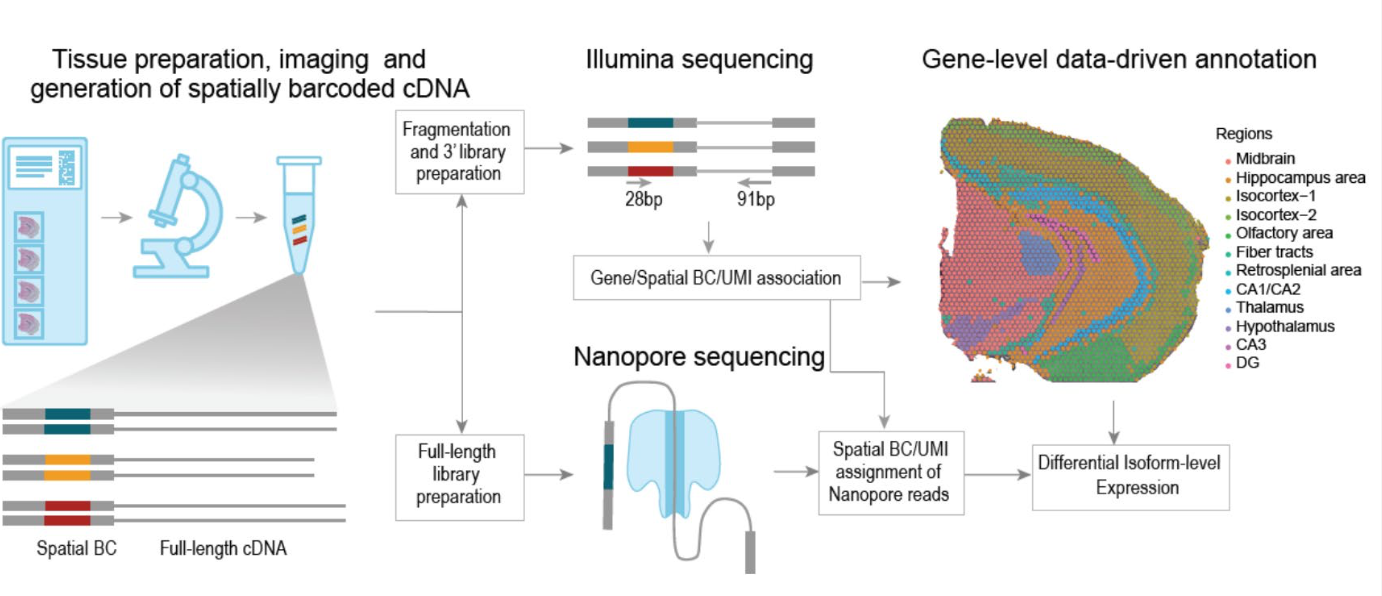
\includegraphics[width=0.5\textwidth]{images/Screenshot_4.png}
\caption{\emph{Lebrigand et al bioRxiv 2022}}
\end{figure}

\hypertarget{dbit-seq-2020}{%
\subsection{DBiT-seq (2020)}\label{dbit-seq-2020}}

Deterministic Barcoding in Tissue, or DBiT-seq, is a method that uses
microfluidics to distribute the barcodes on the tissue slide, rather than
having them pre-spotted on the array. Moreover the technique allows for 
parallel profiling of mRNA and antibody-based protein barcoding.

The procedure is the following:
\begin{itemize}
\tightlist
\item 
  Fix the tissue on the slide
\item
  If performing antibody-based protein barcoding, add antibodies for the
  protein(s) of interest. These antibodies are bound to an RNA sequence
  containing an antibody-derived tag (ADT, just like for CITE-seq) and a
  a ploy-A sequence.
\item 
  Using a microfluidic flow cell with 50 parallel channels, allow 50 
  different barcodes to flow over the tissue slide. These first barcodes, 
  barcodes A, will bind to all poly-A chains (both those from mRNAs and those
  from antibodies). 
\item
  Using a second microfluidic flow cell with 50 parallel channels, placed 
  orthogonally with respect to the first one, 50 barcodes are allowed to
  flow on the tissue slide. These barcodes, barcodes B, will bind to all
  barcodes A. Moreover, barcodes B contain a PCR handle. After this step, 
  all pixels of the slides will be univocally identified by a combination of 
  barcode A + barcode B.
\item 
  Perform imaging steps; this allows to define the position of all pixels 
  on the slide.
\item
  Standard sequencing library preparation.
\end{itemize}

Notice that the same sequences can be used for barcodes A and barcodes B,
since they are always attached in a specific order.
Channel width is what defines the size of the pixel and thus the resolution;
usual channel widths are 50, 25 or 10 $ \mu m$. The number of pixels is the 
square of the number of barcodes meaning, for instance, 2500 spots with a
50x50 grid.

\begin{figure}
\centering
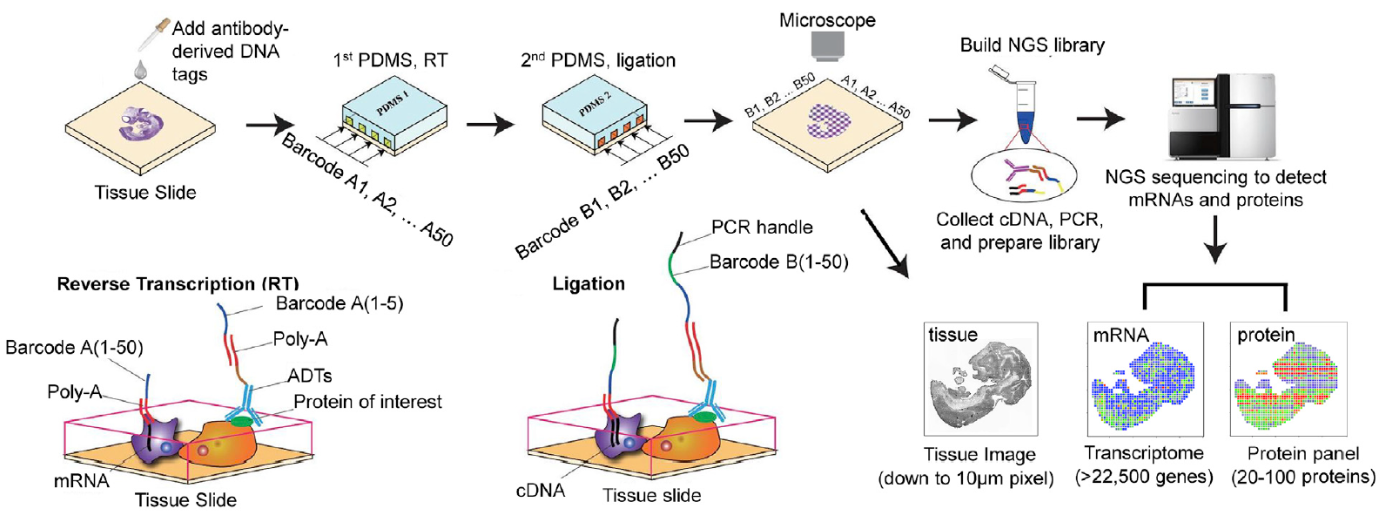
\includegraphics[width=0.5\textwidth]{images/Screenshot_2.png}
\caption{Liu et al., Cell 2020}
\end{figure}

\hypertarget{slide-seq-2019}{%
\subsection{Slide-seq (2019)}\label{slide-seq-2019}}

Slide-seq is akin to spatial transcriptomics in the sense that the tissue
sample is placed on top of the probes; unlike spatial transcriptomics though, 
the probes are not directly spotted on the slide, but rather fixed on top of
10 $\mu m$ diameter beads which are stacked on top of the slide. The probes
have pretty much the same structure as those used in spatial transcriptomics,
where the spatial barcode is bead specific and all the probes on a bead have
different UMIs.

The procedure is the same as spatial transcriptomics but with the different
slide.

Still, even with 10 $\mu m$ beads, one bead could correspond to 1-3 cells.

\begin{figure}
\centering
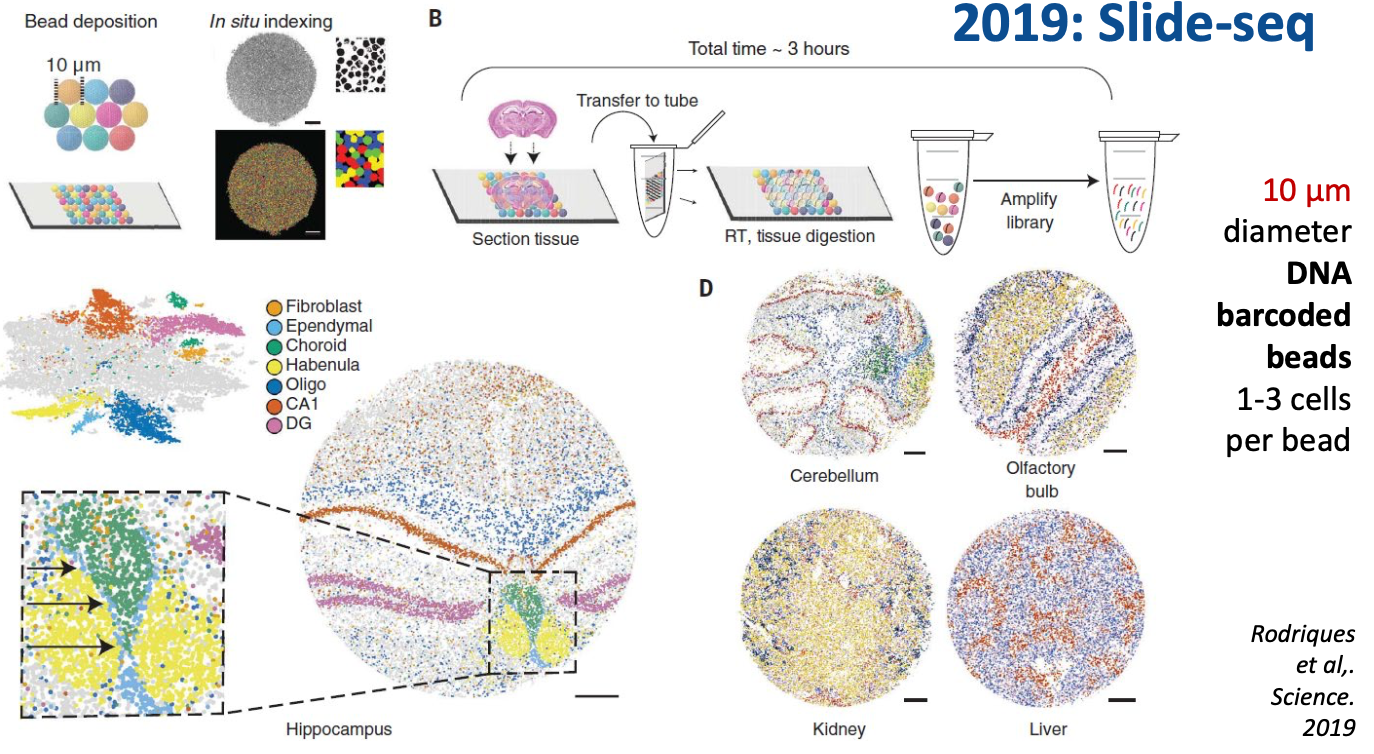
\includegraphics[width=0.5\textwidth]{images/Screenshot_1.png}
\caption{}
\end{figure}

\hypertarget{seq-scope-2021}{%
\subsection{Seq-scope (2021)}\label{seq-scope-2021}}

Seq-scope is a technique that allows for resolution comparable to an optical
microscope (0.5-0.8 $\mu m$ ) by using a repurposed Illumina sequencing 
platform (MiSeq flow-cell in the publication).  

The procedure is as follows:
\begin{itemize}
\tightlist
\item 
  The probes, containing different high-definition map coordinate identifiers,
  or HDMIs, (which are basically spatial barcodes) are hybridized in random 
  positions on the MiSeq flow-cell.
\item 
  The probes undergo the bridge amplification step, therefore forming 
  clusters with one HDMI each. 
\item 
  By using sequencing by synthesis, the position of the clusters on the flow
  cell and the HDMIs of each of them are defined. (Consider the clusters
  as analogous of the spots in other techniques, but randomly placed on the
  slide and with way smaller size).
\item
  The probes are cut in order to expose an oligo-dT tail.
\item
  The fresh frozen tissue (mouse liver sections in the original paper) is 
  placed on top of the flow cell and the cells are permeabilized, allowing 
  for the poly-adenylated RNAs to bind the probes.
\item 
  Imaging steps to define cell positions in the tissue.
\item
  During the second strand synthesis a UMI is included for each molecule.
\item 
  The hybridized probes are detached from the flow cell and PCR adapters are
  added.
\item
  The probes are therefore amplified and sequenced.
\end{itemize}

Given the very small size of the clusters, the technique allows for 
sub-cellular resolution; each cluster will contain only the RNAs from a 
region of the original cell.

\begin{figure}
\centering
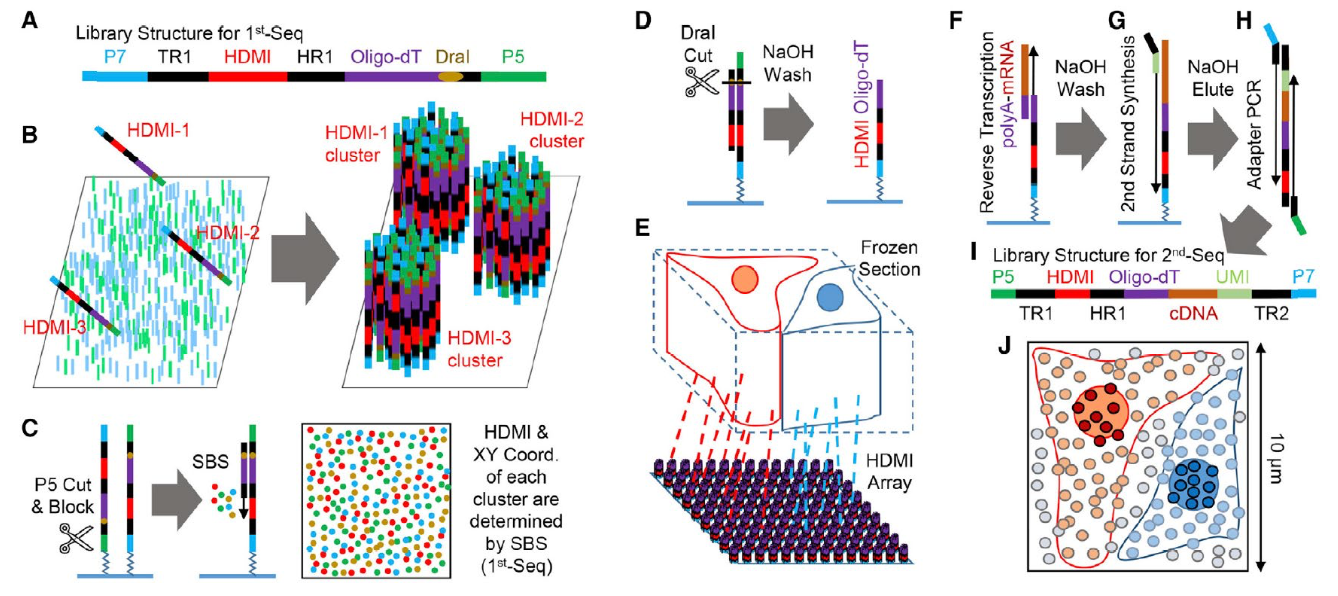
\includegraphics[width=0.5\textwidth]{images/Screenshot_3.png}
\caption{\emph{Cho et al., Cell 2021}}
\end{figure}

\hypertarget{imaging-based-methods}{%
\section{Imaging based methods}\label{imaging-based-methods}}

\hypertarget{in-situ-hybridization}{%
\subsection{In-Situ Hybridization}\label{in-situ-hybridization}}

ISH (In Situ Hybridization) is based on nucleic acid probes synthesized,
\textbf{labeled}, purified, and annealed with the specific target (by
complementarity). The technique can be applied to DNA and RNA with
nucleic acid probes (20-50long).

\hypertarget{radioactive-ish-1967}{%
\subsubsection{Radioactive ISH (1967)}\label{radioactive-ish-1967}}

ISH was first used to study the formation and detection of RNA-DNA
hybrid molecules in cytological preparations (\emph{Gall and Pardue,
PNAS,1969}).  Cells are treated in order to denature DNA and
incubated with RNA to detect hybrids by \textbf{autoradiography}. Probes
are able to catch radioactivity signal and are identified where the
ribosomes are being produced.

\hypertarget{fish-1997}{%
\subsubsection{FISH (1997)}\label{fish-1997}}

\begin{itemize}
\tightlist
\item
  \textbf{Direct FISH detection:} fluorescent labels attached to the
  probe which will hybridize to a target DNA/RNA
\item
  \textbf{Indirect FISH detection:} biotin is attached to the probe.
  Streptavidin linked to a fluorescent tag binds biotin with high
  specificity.
\end{itemize}

Fluorescence microscopy can be used to find out where the fluorescent
probe is bound.

\hypertarget{whole-mount-ish-1989}{%
\subsubsection{\texorpdfstring{\textbf{Whole mount ISH
(1989)}}{Whole mount ISH (1989)}}\label{whole-mount-ish-1989}}

Whole mount in situ hybridization determines the RNA expression pattern
of a gene in the context of a whole embryo or embryo piece/organ (also
3D). First experiments were carried out already knowing the pattern of
expression of certain genes. They selected:

\begin{enumerate}
\def\labelenumi{\arabic{enumi}.}
\tightlist
\item
  hunchback
\item
  krippel
\item
  knirps
\item
  fushi tarazu
\end{enumerate}

They could also look at how different was the localization between mRNA
and proteins produced, with antibodies.

\hypertarget{rna-smfish-2002}{%
\subsubsection{\texorpdfstring{RNA \textbf{smFISH
(2002)}}{RNA smFISH (2002)}}\label{rna-smfish-2002}}

The release of the first reference genomes, allowed the computational
design of probes. Multiple probes can be used for a single transcript
for increased specificity and single molecule resolution. Each probe is
labeled with different labels. The combination of ``colors'' forming a
pseudocolor is assigned to a specific transcript.

For smFISH, they used 4 different fluorophores for the identification of
10 genes. smFISH has a problem: the number of combinations (pseudogenes)
is limited by the number of probes. This was solved by the next
technique.

\begin{figure}
\centering
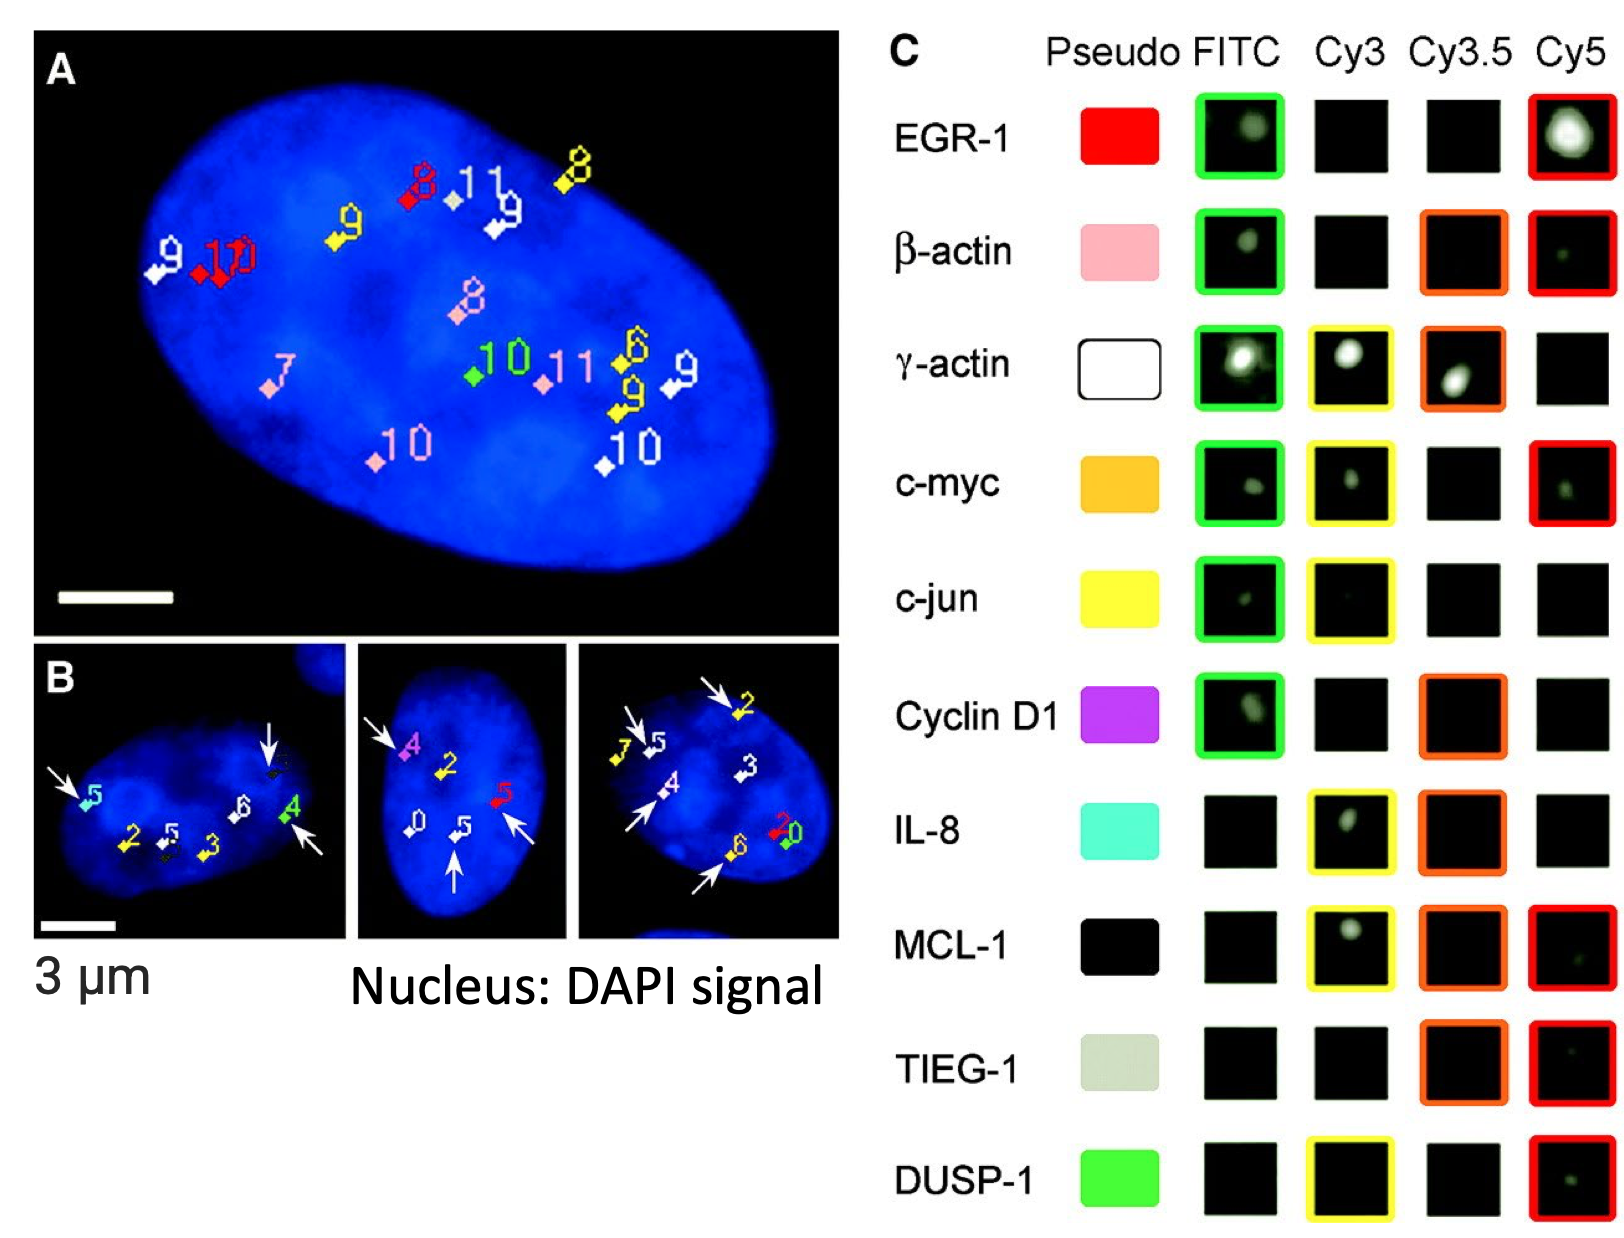
\includegraphics[width=0.5\textwidth]{images/Screenshot_5.png}
\caption{\emph{Levsky et al, Single-Cell Gene Expression Profiling,
Science 2002}}
\end{figure}

\hypertarget{merfish-2015}{%
\subsubsection{\texorpdfstring{\textbf{MERFISH
(2015)}}{MERFISH (2015)}}\label{merfish-2015}}

Multiplexed Error-Robust FISH (MERFISH) is based on multiple rounds of
hybridization and detection of signal, with consequent removal of probe
for each round. The barcode is formed by checking at each round if the
signal of the probe you are expecting is present on an RNA molecule
(N-bit binary code: if yes, bit signal 1, else 0). They use an indirect
method with two types of probes, one type that binds to RNA and one that
binds to the fluorophore.

\begin{figure}
\centering
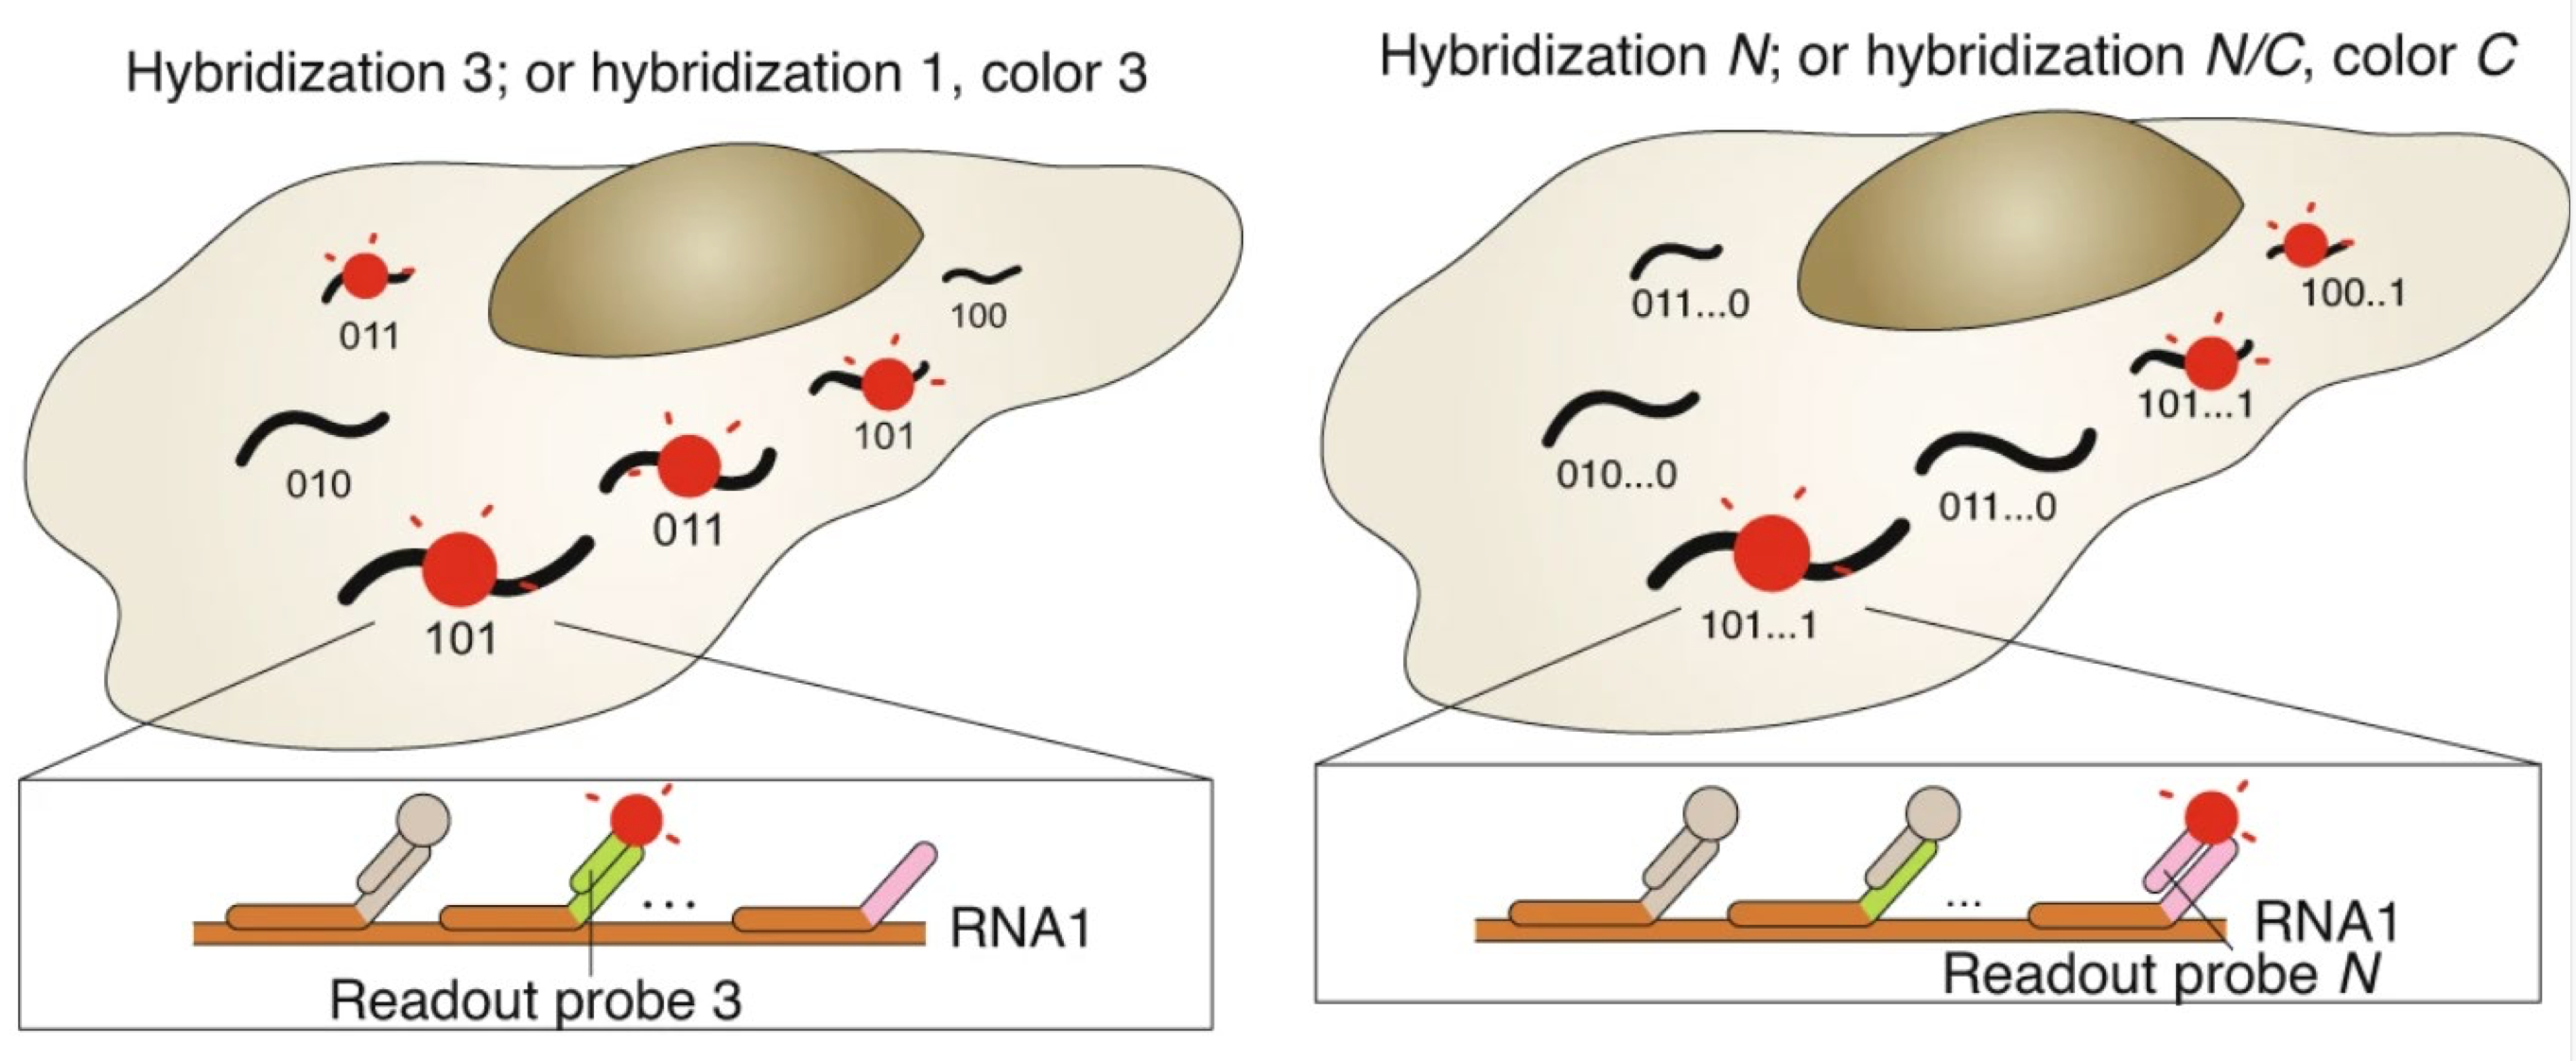
\includegraphics[width=0.5\textwidth]{images/Screenshot_6.png}
\caption{\emph{Chen et al, Science 2015}}
\end{figure}

Encoding-readout labeling strategy allows genome-scale imaging with
shorter experimental duration hybridization of FISH probes to
exogenously introduced readout sequences is much faster than
hybridization directly to cellular RNAs. The binary coding scheme (1
color) distinguishes 2N genes with N rounds of hybridization. When C
colors are used, 2NC genes can be distinguished with N hybridization
rounds.

Analysis example: simultaneous measurement of 140 RNA species in a
single cell (IMR90, fibroblast). MERFISH with a 16-bit MHD4 code
(modified humming distance 4 code) at least four bits must be read
incorrectly to change one valid codeword into another). Error detection
\& correction.

\hypertarget{rna-seqfish-2019}{%
\subsubsection{\texorpdfstring{\textbf{RNA seqFISH+
(2019)}}{RNA seqFISH+ (2019)}}\label{rna-seqfish-2019}}

80 rounds of hybridization with 3 color imaging (identified 47k mRNA).
Tried in mouse brain slices and identified the position of transcripts
with respect to all the others, in different types of cells. Is it also
possible to then build the architecture of the tissue, in terms of what
kind of cells appear close to others.

\begin{figure}
\centering
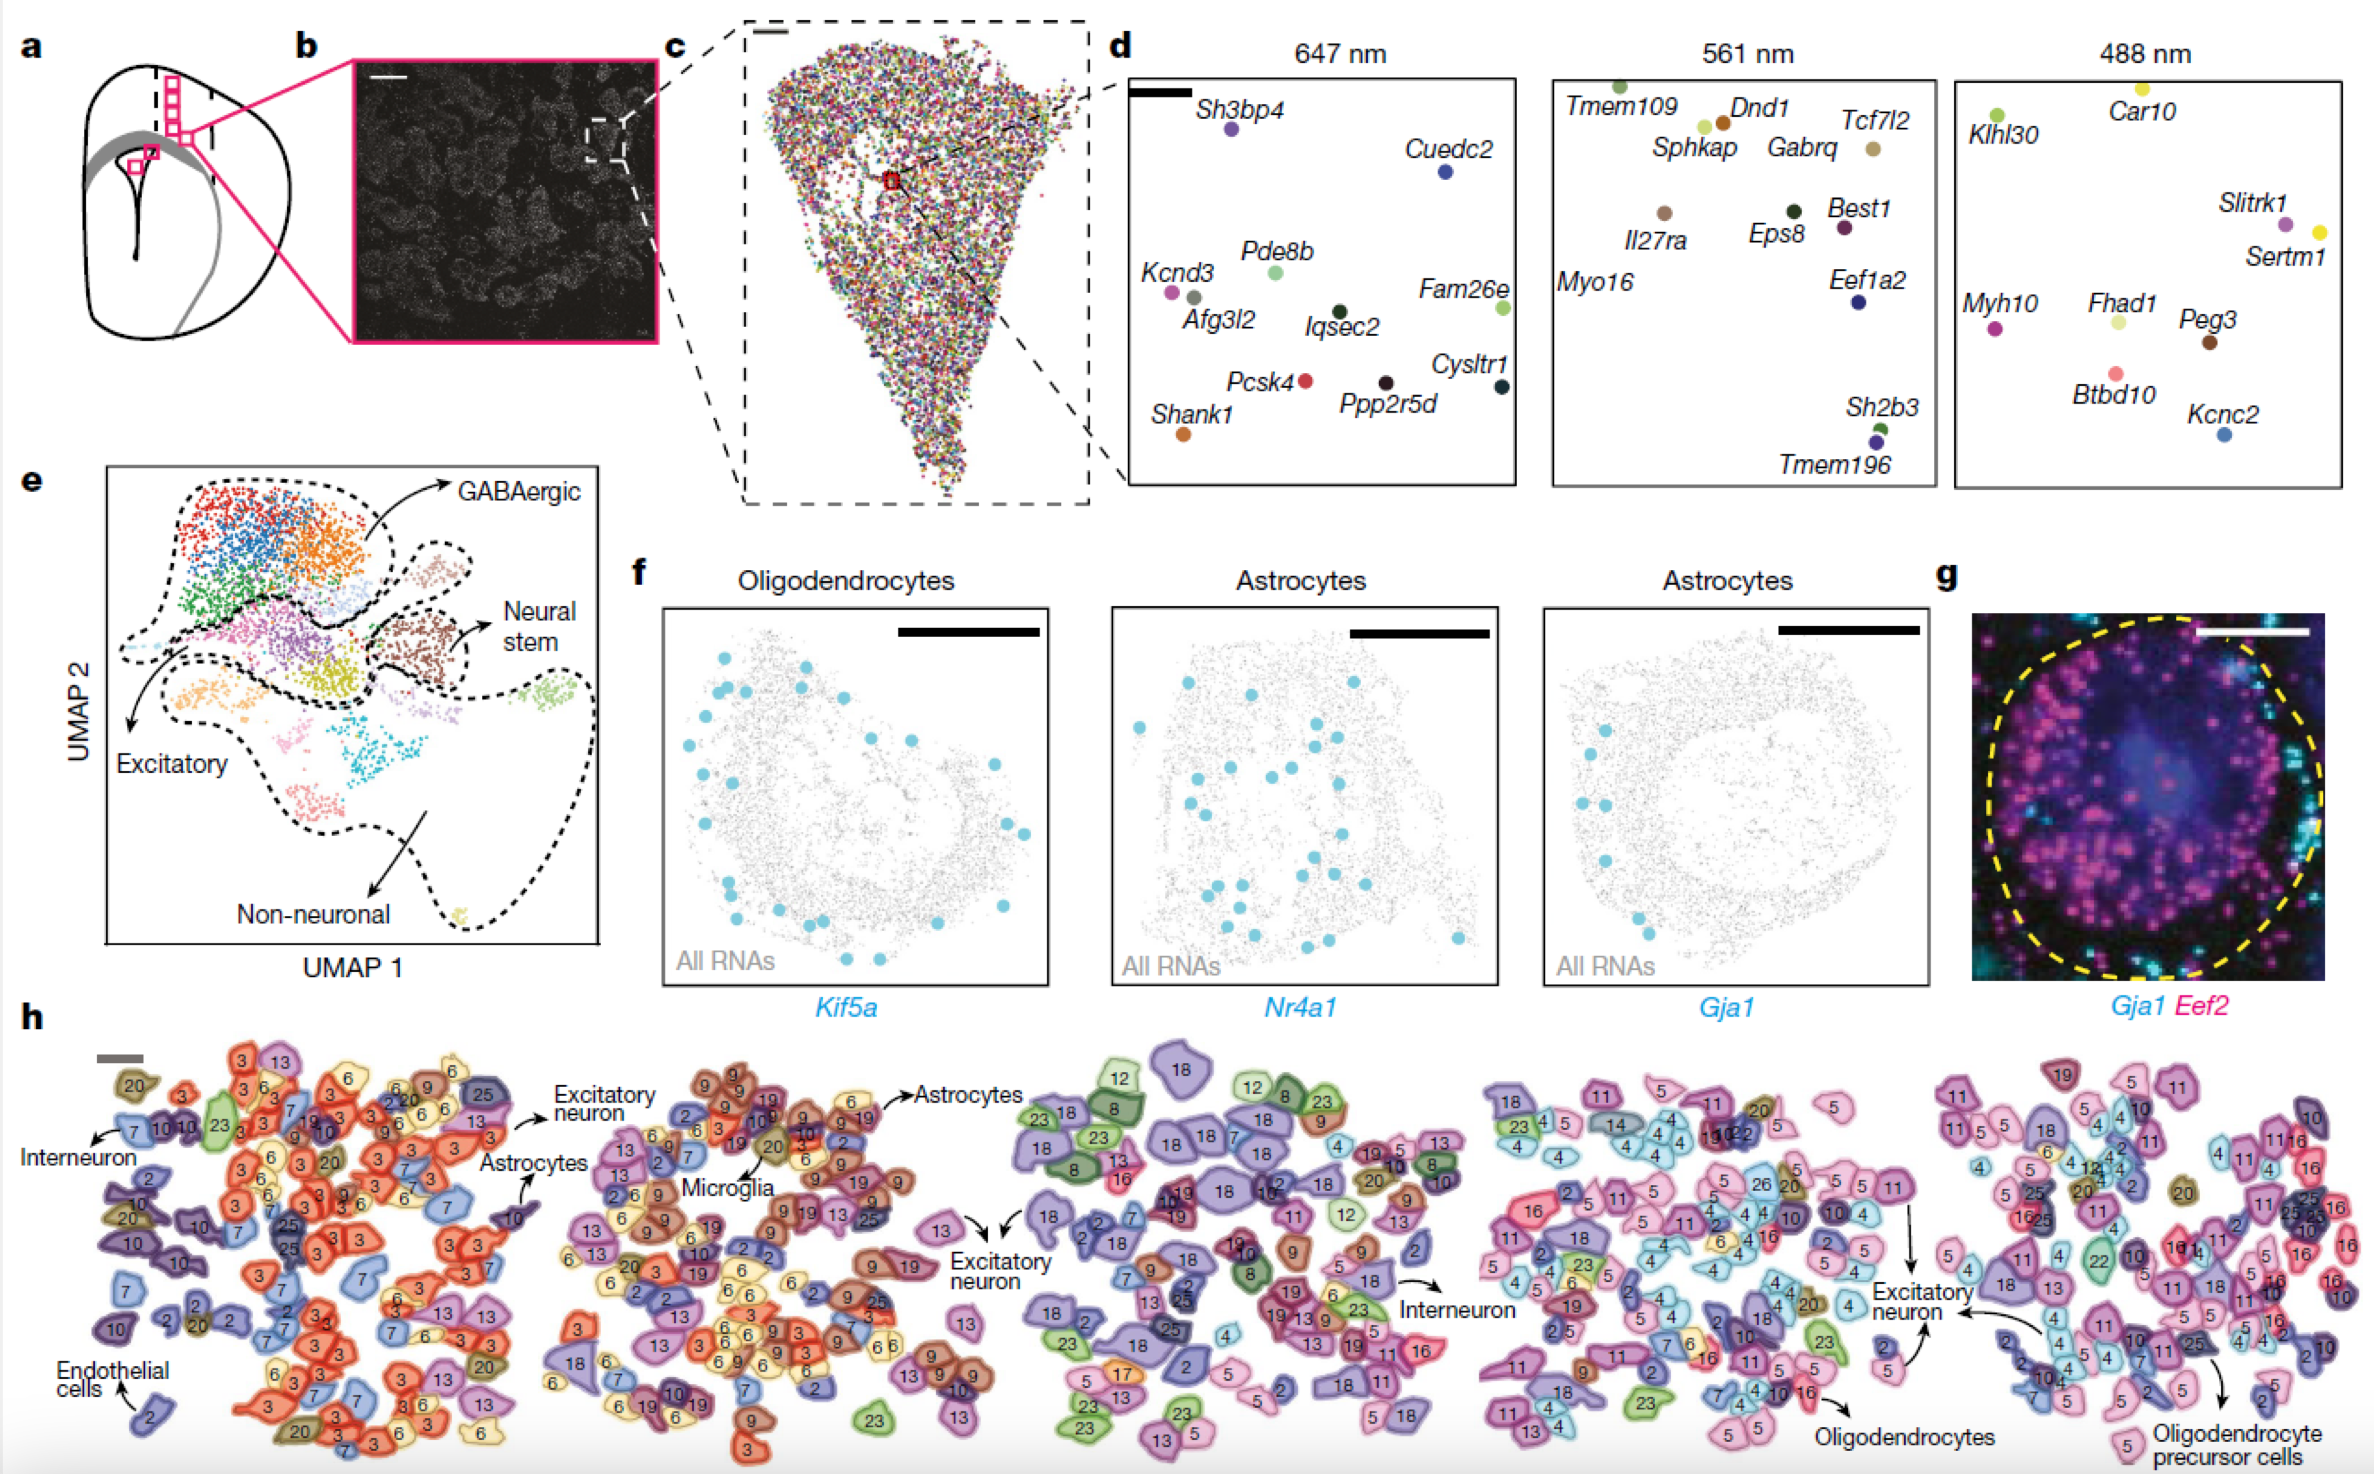
\includegraphics[width=0.5\textwidth]{images/Screenshot_7.png}
\caption{}
\end{figure}

\hypertarget{merscope-platform-2021}{%
\subsubsection{MERSCOPE platform (2021)}\label{merscope-platform-2021}}

Commercial platform using MERFISH technology. It is possible to study
spatial features at different resolution levels:

\begin{itemize}
\tightlist
\item
  whole section (9x7 mm) e.g.~tissue organization
\item
  wide field of view (200x200 micron) e.g.~cell interaction or function
\item
  sub-cellular (12x12 micron, equivalent to \textless{} 100 nm) e.g.~L2
  or 3 IT Glutamatergic neuron
\end{itemize}

Vizgen MERSCOPE automatically segments the cells in the MERFISH
measurement using a segmentation method called Baysor, that optimizes
cell boundaries considering joint likelihood of transcriptional
composition and cell morphology (size and shape of the cell). The
approach can take into account \textbf{nuclear (DAPI) or cytoplasm
(poly(A)) staining}, however, can also perform segmentation based on the
detected molecules alone. By tuning parameters, a better visualization
can be obtained e.g.~alpha for transparency, palette, etc. Using the
positional information of each cell, we compute spatial niches (region
of tissue). A relevant aspect into account is the doublet rate
i.e.~mixture of cell types in the same pixel.

\hypertarget{x-xenium-platform-2023}{%
\subsubsection{\texorpdfstring{\textbf{10x Xenium platform
(2023)}}{10x Xenium platform (2023)}}\label{x-xenium-platform-2023}}

Probes are designed in a slightly different way: they have two
complementary arms that, if close to each other, can undergo a process
of \textbf{ligation} (this allows to rule out the fact that the probe
might bind to two different mRNA molecules).

\hypertarget{akoya-platform-2021}{%
\subsubsection{AKOYA platform (2021)}\label{akoya-platform-2021}}

The CODEX platform developed by Akoya Biosciences is based on DNA
barcoded antibodies, which allow to perform multiplexed imaging.
Antibodies are specific for one protein, and the addition of fluorescent
probes complementary to the DNA barcode (antibody specific) allow the
visible rendering of the antibody. After signal detection, chemical
stripping of fluorescent oligonucleotides occurs. The difference with
previous techniques is that we capture proteins instead of transcripts.

\hypertarget{summary}{%
\subsection{Summary}\label{summary}}

\textbf{Improvements:}

\begin{itemize}
\tightlist
\item
  Throughput (up to 1000s different RNAs)
\item
  High resolution (subcellular)
\item
  No polyA restriction (but sequence and splicing knowledge necessary to
  design complementary probes)
\end{itemize}

\textbf{Challenges:}

\begin{itemize}
\tightlist
\item
  optical resolution (microscope)
\item
  density \& structure of transcripts in cells (RNA granules,
  RNA-protein interactions could compromise probe hybridization)
\end{itemize}

\hypertarget{spatial-omics-analysis}{%
\section{Spatial omics analysis}\label{spatial-omics-analysis}}

\hypertarget{deconvolution-of-low-resolution-multi-cell-spots}{%
\subsection{Deconvolution of low-resolution multi-cell
spots}\label{deconvolution-of-low-resolution-multi-cell-spots}}

The aim is to uncover cellular heterogeneity in low resolution spots
(e.g.~Visium) to disentangle the spatial patterns of cell types. Most
methods rely on the availability of a single cell annotated reference.

\begin{itemize}
\tightlist
\item
  understand how many nuclei are present in a spot
\item
  analyze cell types present in each spot
\end{itemize}

In \emph{Li et al.~Nature Communications. 2023} 18 different
deconvolution methods are compared. The composition of the spot is
represented as a pie chart.

\begin{figure}
\centering
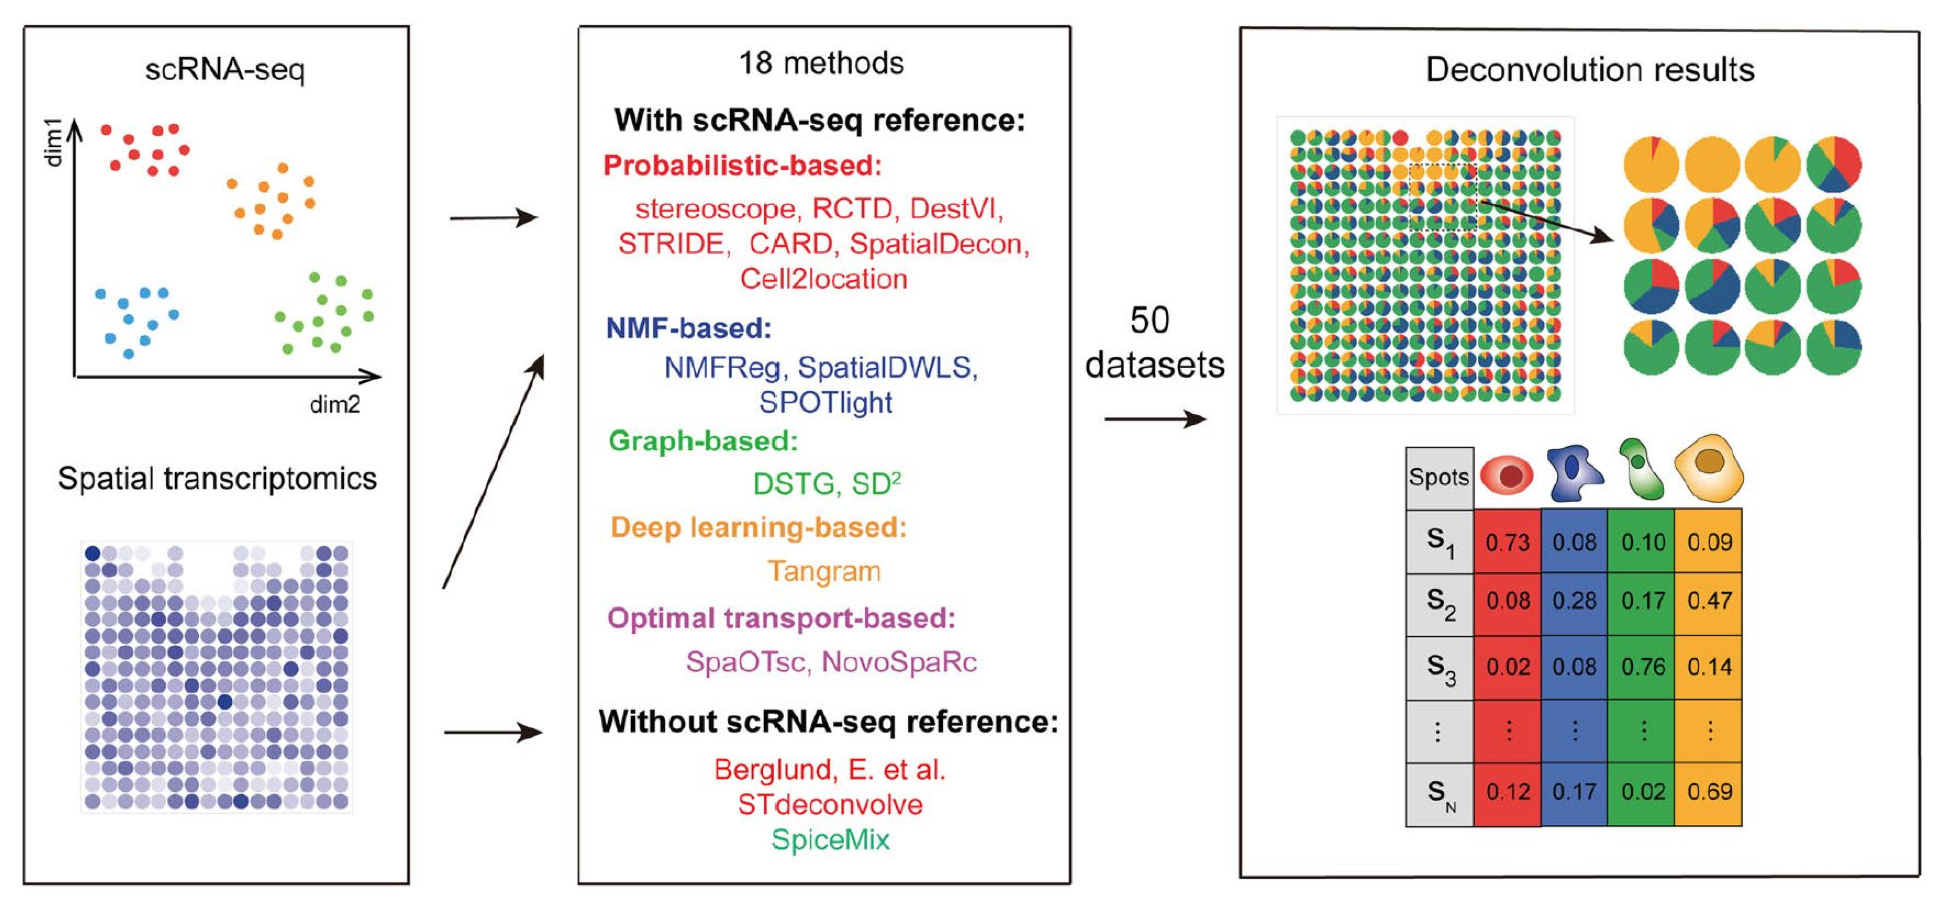
\includegraphics[width=0.5\textwidth]{images/Screenshot_8.png}
\caption{\emph{Li et al.~Nature Communications. 2023}}
\end{figure}


The best performing method is CARD, tool published in 2022 based on
matrix factorization. A single cell reference or matrix of gene
expression data is required (for cell marker identification) and the
location of the spots from spatial transcriptomics. The final results
will report the estimated cell type proportion.

\begin{figure}
\centering
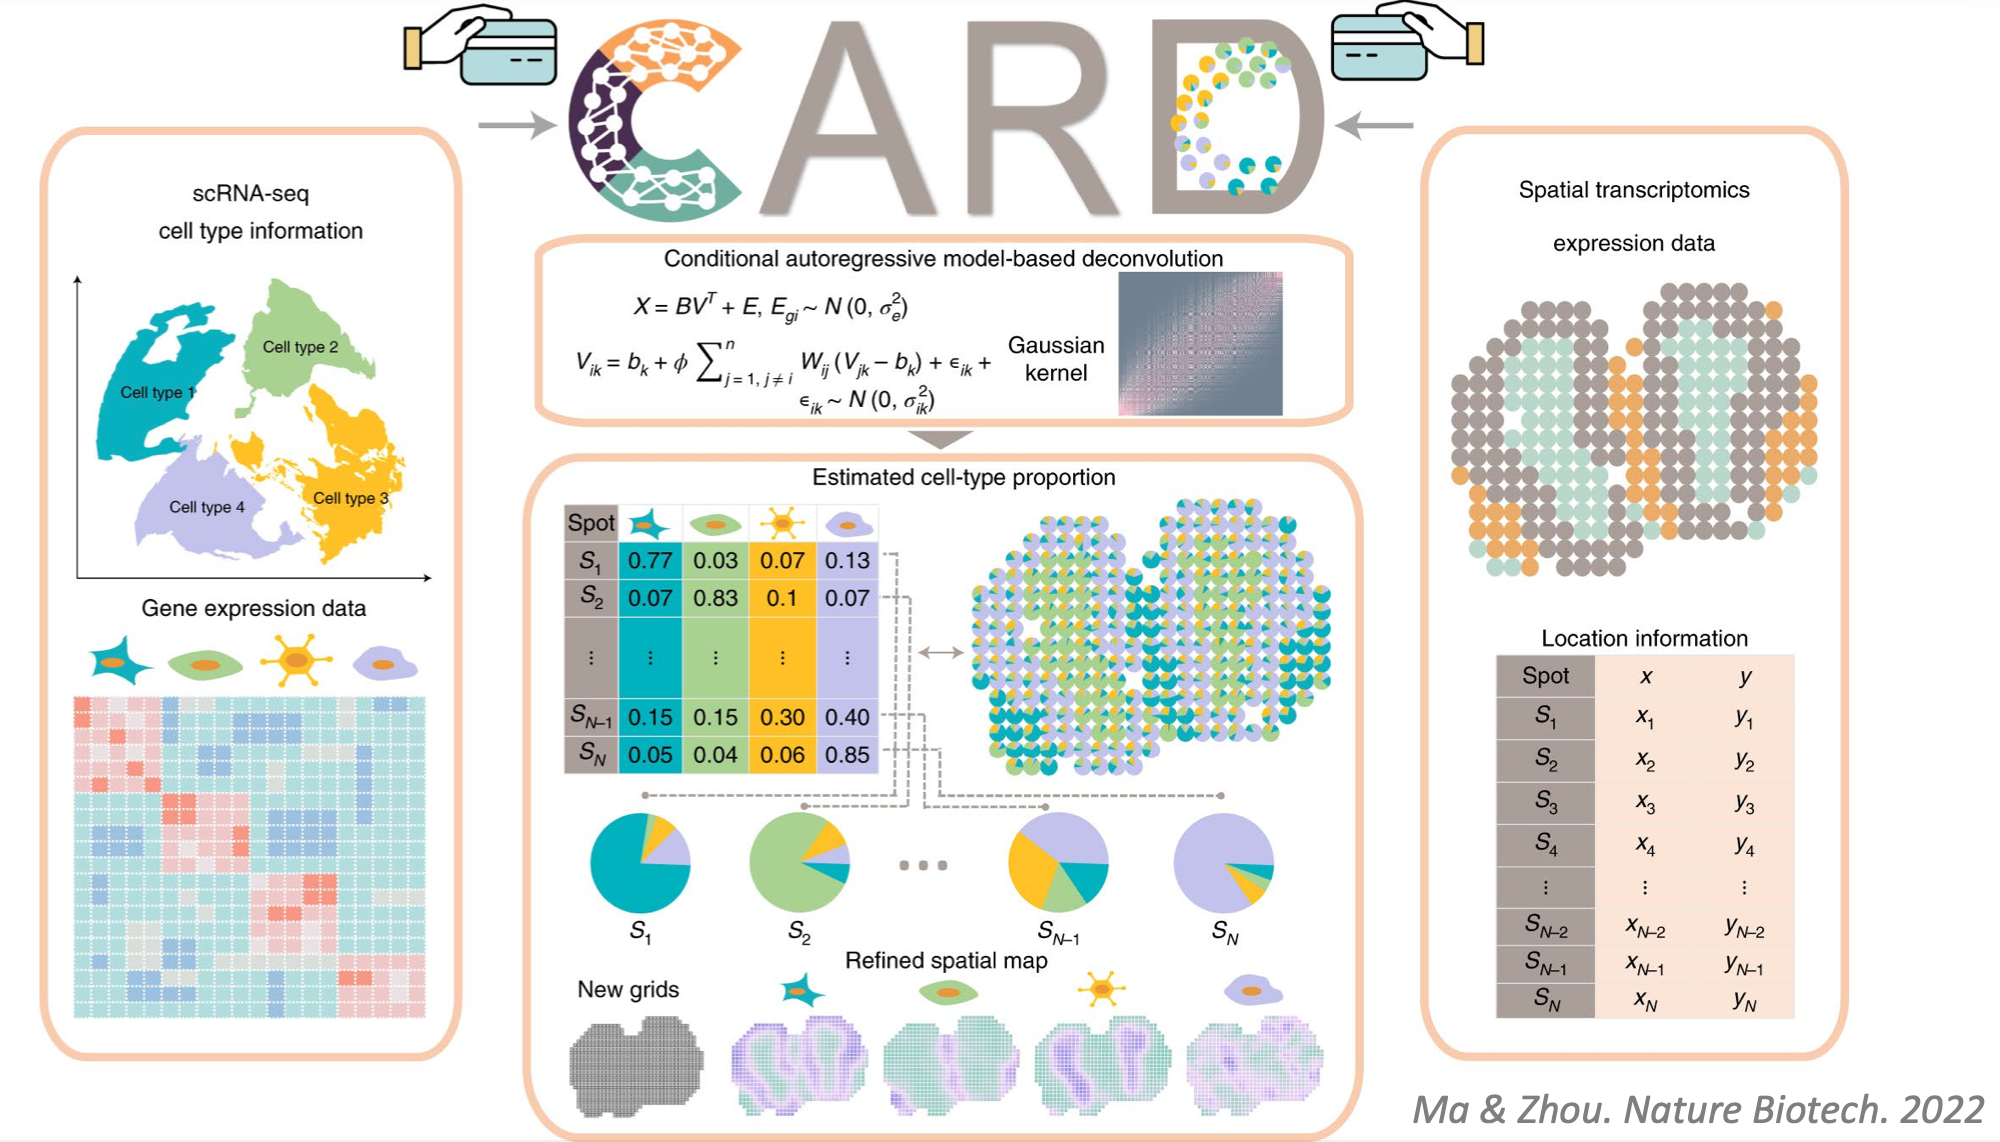
\includegraphics[width=0.5\textwidth]{images/Screenshot_9.png}
\caption{}
\end{figure}

\hypertarget{cell-segmentation-in-imaging-based-methods}{%
\subsection{Cell segmentation in imaging-based
methods}\label{cell-segmentation-in-imaging-based-methods}}

Analysis specific for imaging approaches. \textbf{Baysor} is applied to
distinguish the boundaries of individual cells based on:

\begin{itemize}
\tightlist
\item
  Co-staining information

  \begin{itemize}
  \tightlist
  \item
    nuclei (for example, DAPI) - most common approach
  \item
    cell bodies (for example, polyA)
  \item
    cellular membranes
  \end{itemize}
\item
  Spatial expression data

  \begin{itemize}
  \tightlist
  \item
    increased spatial density of molecules within cell somas
  \item
    transcriptional composition of local molecular neighborhoods
  \end{itemize}
\end{itemize}

\hypertarget{inference-of-cell-cell-communication}{%
\subsection{Inference of Cell-cell
communication}\label{inference-of-cell-cell-communication}}

Reconstruct cell-cell communication from single-cell and/or spatial
omics. The idea behind this is studying how cells react to stimuli from
their environment(in multicellular organisms, other cells) relevant for
apoptosis and cell migration, essential in homeostasis and disease.
Ligands (soluble proteins) bind to receptors on the cell surface,
activating cascade affecting transcriptional regulation.

\begin{figure}
\centering
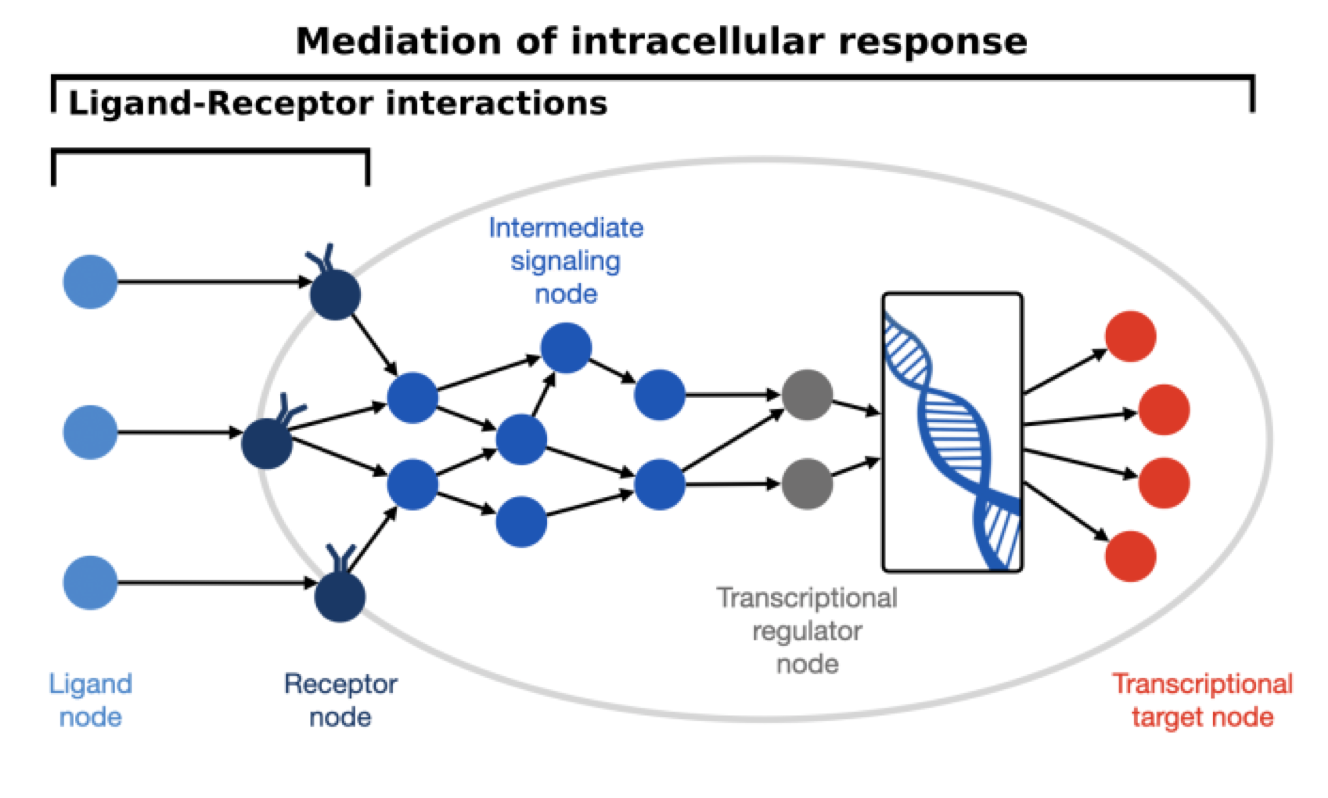
\includegraphics[width=0.5\textwidth]{images/Screenshot_10.png}
\caption{}
\end{figure}

\hypertarget{cellphonedb}{%
\subsubsection{CellPhoneDB}\label{cellphonedb}}

The method infers crosstalk between pairs of cell groups (source and
receiver) and is mainly based on expression of \textbf{ligands} (by the
source) and \textbf{receptors} (on the receiver). Information about
ligand-receptor interactions extracted from prior knowledge resources
e.g.~PPI-interaction, protein complexes and secreted or membrane
proteins databases.

Enriched receptor--ligand interactions are identified from the average
expression of a ligand (source) and a receptor (target). Assumption:
expression levels match protein levels. The method can be used in
multiple conditions to study how communication changes upon stimuli or
in disease settings.

\hypertarget{integration-between-single-cell-and-spatial-omics}{%
\subsection{Integration between single cell and spatial
omics}\label{integration-between-single-cell-and-spatial-omics}}

In order to perform a comprehensive study, it is possible to combine
multimodal spatial omics e.g.~DbitSEQ to combine epigenome and
transcriptome.

\hypertarget{spatal-omics-reference-atlases}{%
\subsection{Spatal omics reference
atlases}\label{spatal-omics-reference-atlases}}

\begin{itemize}
\tightlist
\item
  BICCN: diverse cell types in human, mouse and non-human primate
  \textbf{brain}
\item
  HuBMAP: global atlas of human body
\item
  Human Cell Atlas: map every cell type of the human body
\item
  Spatial Omics DataBase (SODB):
\end{itemize}
